\section{Evaluation}
\label{sec-evaluation}

%Metrics: what do you care about?
%Evaluation methodology: how did you evaluate?
%Results / discussions: if possible, provide intuitions and reasons for the
%result you got.

As described in the previous section, our study focuses on analyzing the AC and
DC power consumption ratios. Intuitively we would expect that DBI-AC and DBI-DC
help the AC and DC power consumption factors respectively. Table
\ref{table:dbi-ratios} illustrates the AC and DC ratio reductions for load and
store operations separately. The average ac/dc ratio improvements were computed
using the following formula:

$$ \TT{\% Improvement} = |\frac{\TT{DbiRatio} - \TT{nonDbiRatio}}{\TT{nonDbiRatio}}| \times 100\%$$

\begin{table}[!htb]
  \centering
    \begin{tabular}{| c | c |}
      \hline
      \textbf{DBI Ratio} & \textbf{\% Improvement} \\ \hline
     Load DC  & 68.59 \\ \hline
     Load AC  & 8.62  \\ \hline
     Store DC & 75.04 \\ \hline
     Store AC & 3.38  \\ \hline
    \end{tabular}
    \caption{Average AC/DC ratio reduction for load and store operations using
    DBI across all 28 MiBench applications}
    \label{table:dbi-ratios}
\end{table}

We can see the DBI-DC reduces the DC factor by 68.6 \% and 75.0 \% for load and
store operations whereas DBI-AC has a smaller reduction of 8.6 \%
and 3.4 \% respectively. Since the DC factor optimized the data values to
reduce the number of binary $0$'s \cite{low-power-dram}, we can conclude that
the values on cache misses for both load and store operations were
predominantly $0$'s  in the MiBench suite. This suggests that DBI, especially
DBI-DC does indeed improve the AC and DC power consumption ratios for
unencrypted memory systems. Next we compare DBI's impact on unencrypted versus
encrypted memory systems.

\begin{figure}[!htb]
  \centering
  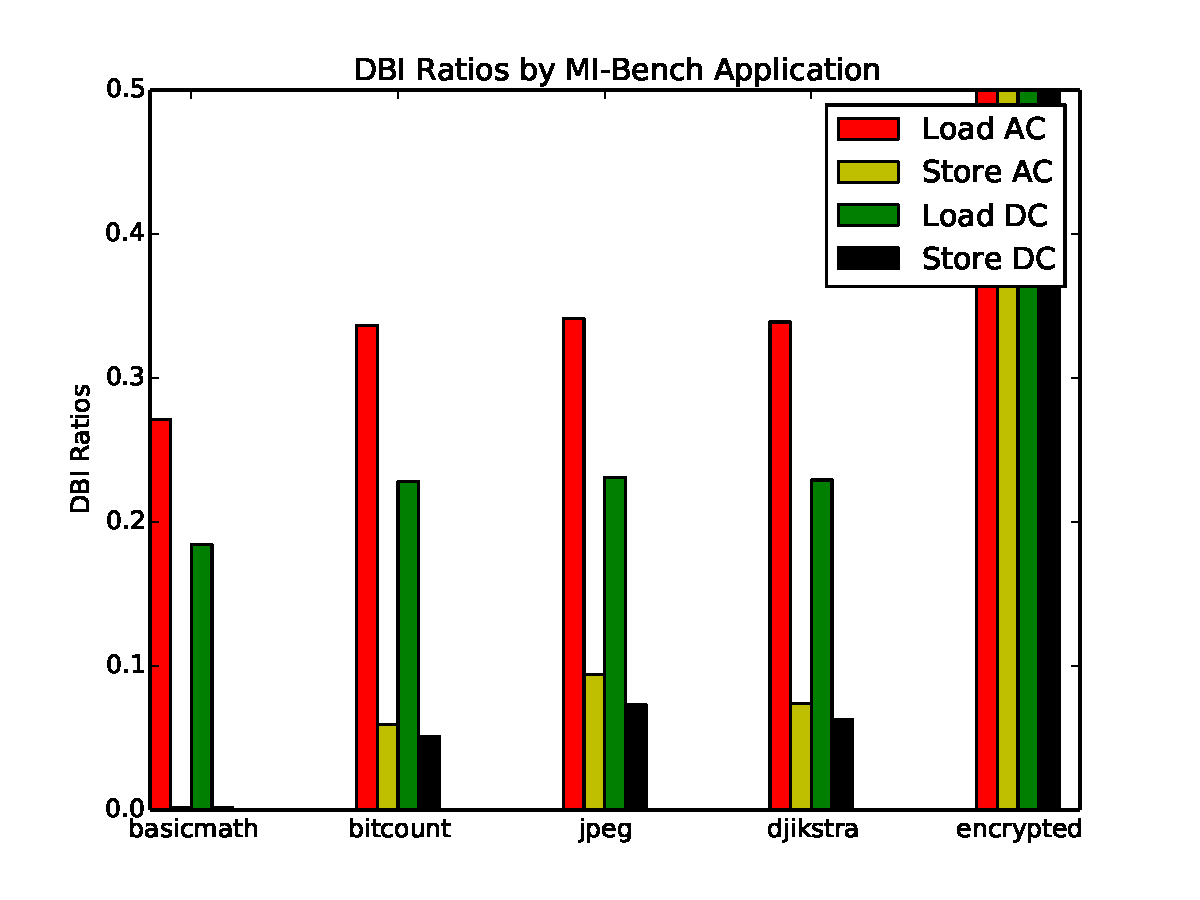
\includegraphics[width=0.5\textwidth]{figs/dbiGraph}
  \caption{Comparing load/store DBI ratios for representative MiBench applications}
  \label{fig:dbiGraph}
\end{figure}

Figure \ref{fig:dbiGraph} illustrates the DBI-AC and DBI-DC ratios for select
MiBench applications and our encrypted system model. The MiBench applications
chosen: \TT{basicmath}, \TT{jpeg}, \TT{djikstra}, \TT{fft}, \TT{bitcount},
\TT{blowfish}, and \TT{strsearch} span all six application classes of MiBench:
\TT{automotive}, \TT{consumer}, \TT{security}, \TT{office}, \TT{telecomm} and
\TT{network}. We chose these specific applications as they span all six
application classes of MiBench and are representative of the memory access
patterns for each of their domains.

\paragraph{Encryption Model} First, the encryption model exhibited DBI-AC and
DBI-DC ratios of 0.5 for both loads and stores. As mentioned in
Section~\ref{sec-methodology}, truly random data exhibits DBI-AC and DBI-DC
ratios of 0.5 \cite{hollis} since truly random data has equal signal
probabilities of 0 and 1, and equal switching probabilities (flip or not flip).
According to the Avalanche effect, changing even a single bit in the
unencrypted plaintext should cause the encrypted ciphertext to appear
completely random \cite{avalance}. Under the avalance effect, we assume
encrypted data is truly random for the purposes of this study. Furthermore, as
shown in Figure \ref{fig:sys-arch}, all cache misses are first encrypted with
the \TT{Encryption Core} before being processed by the off-chip DRAM based
memory system. This means that for the encrypted model, all data seen by the
DDR4 DRAM memory system will be truly random and DBI-AC and DBI-DC ratios will
be 0.5. Though the true DBI-AC and DBI-DC ratios may be less than 0.5, we
believe that the difference would not be significant enough to change the
underlying results of this study.

As seen in Figure \ref{fig:dbiGraph}, the DBI-AC and DBI-DC ratios for load and
store operations for the MiBench applications is significantly lower than that
of encrypted model. This suggests that for unencrypted data stores and loads
that follow the MiBench memory access pattern, DBI-AC and DBI-DC can
significantly reduce the AC and DC power factors to 0.33 for Load-AC,
0.07 for Store-AC, 0.22 for Load-DC and 0.06 for Store-DC on average across all
MiBench applications. If the encryption scheme seen in Figure
\ref{fig:sys-arch} were used, the DBI-AC and DBI-DC ratios would be 0.5. This
suggests that for load and store operations, encryption would incur a
significant power overhead.

Interestingly, we see that for all MiBench applications --- especially the
select ones shown in Figure \ref{fig:dbiGraph} --- the load and store ratios
are relatively consistent. This can be explained by the fact that for the given
cache architecture, the MiBench applications may have similar miss rates per
1000 instructions \cite{mibench}. From the select applications, \TT{rijindael}
and \TT{ispell}, and the given cache configuration : 32KB size, 8 way
associative and 128B cache lines both applications have around 3 misses per
1000 instructions. Assuming that the trend continues for the all applications
in the MiBench suite, the DBI ratio similarity across the applications is
expected. Furthermore, it should be noted that MiBench is organized such that
each application has two version: \TT{small-input} and \TT{large-input}. We
noticed that for all applications, the small and large input version exhibited
virtually the same DBI ratios which can also be explained by the fact that
despite the varying input data sets, the memory access pattern should be the
same across both versions resulting in similar DBI ratios.
